%!TEX encoding = UTF-8 Unicode
%!TEX root = ../livre-can.tex

%-----------------------------------------------------------------------------------------------------
%   DESSIN TRAME CAN
%-----------------------------------------------------------------------------------------------------

\newcommand\startcanbit{\pgfmathparse{0}\let\x\pgfmathresult}

\newcommand\cancommentstyle{\scriptsize}
\newcommand\cantextstyle{\scriptsize\tt}
\newcommand\canbitwidth{.7}
\newcommand\canbitheight{.5}

\newcommand\canbitstyle{[thick, fill=lightgray!25]}

\newcommand\canspace[1]{
  \pgfmathparse{\x + \canbitwidth * #1}\let\x\pgfmathresult
}
\newcommand\canbit[1]{
  \draw (\x, 0)\canbitstyle rectangle ++ (\canbitwidth, \canbitheight) ;
  \draw (\x + \canbitwidth * 0.5, \canbitheight * 0.5) node {\cantextstyle #1} ;
  \pgfmathparse{\x + \canbitwidth}\let\x\pgfmathresult
}

\newcommand\canbitfield[1]{
  \draw (\x, 0)\canbitstyle rectangle ++ (3 * \canbitwidth, \canbitheight) ;
  \draw (\x + \canbitwidth * 1.5, \canbitheight * 0.5) node {\cantextstyle #1} ;
  \pgfmathparse{\x + 3 * \canbitwidth}\let\x\pgfmathresult
}

\newcommand\canbitl[1]{
  \draw (\x, 0)\canbitstyle -- ++ (0, \canbitheight) ;
  \draw (\x, 0)\canbitstyle -- ++ (\canbitwidth, 0) ;
  \draw (\x + \canbitwidth * 0.5, \canbitheight * 0.5) node {\cantextstyle #1} ;
  \pgfmathparse{\x + \canbitwidth}\let\x\pgfmathresult
  \draw (\x, 0)\canbitstyle -- ++ (0, \canbitheight) ;
}

\newcommand\cangraybitlow[1]{
  \fill[lightgray!25] (\x, 0) rectangle (\x + \canbitwidth, \canbitheight) ;
  \canbitl{#1}
}

\newcommand\canbith[1]{
  \draw (\x, 0)\canbitstyle -- ++ (0, \canbitheight) ;
  \draw (\x, \canbitheight)\canbitstyle -- ++ (\canbitwidth, 0) ;
  \draw (\x + \canbitwidth * 0.5, \canbitheight * 0.5) node {\cantextstyle #1} ;
  \pgfmathparse{\x + \canbitwidth}\let\x\pgfmathresult
  \draw (\x, 0)\canbitstyle -- ++ (0, \canbitheight) ;
}

\newcommand\cangraybithigh[1]{
  \fill[lightgray!25] (\x, 0) rectangle (\x + \canbitwidth, \canbitheight) ;
  \canbith{#1}
}
\newcommand\canidle{
  \draw (\x, 0)\canbitstyle -- ++ (0, \canbitheight) ;
  \draw (\x, \canbitheight)\canbitstyle -- ++ (3 * \canbitwidth, 0) ;
  \draw (\x + \canbitwidth * 1.5, \canbitheight * 0.5) node {\cantextstyle \dots} ;
  \pgfmathparse{\x + 3 * \canbitwidth}\let\x\pgfmathresult
  \draw (\x, 0)\canbitstyle -- ++ (0, \canbitheight) ;
}

\newcommand\candots{
  \draw (\x, 0)[dotted]\canbitstyle -- ++ (\canbitwidth, 0) ;
  \draw (\x, \canbitheight) [dotted]\canbitstyle -- ++ (\canbitwidth, 0) ;
  \pgfmathparse{\x + \canbitwidth}\let\x\pgfmathresult
}

%-----------------------------------------------------------------------------------------------------

\chapter{Protocole CAN}

%--- Pour supprimer tout en-tête et pied de page sur la 1re page d'un chapitre
\thispagestyle{empty}


\begin{figure}[h!]
  \centering
  \begin{tikzpicture}[transform shape, rotate=90]
    \draw (3 * \canbitwidth, -2 + .5 * \canbitheight) node[left]{\cancommentstyle Standard} ;
    \draw (3 * \canbitwidth, -4 + .5 * \canbitheight) node[left]{\cancommentstyle Étendue} ;
    \draw ( 2 * \canbitwidth, 0)[dotted] -- ++ (0, 4) ;
    \draw ( 3 * \canbitwidth, -4.5)[dotted] -- (3 * \canbitwidth, 1.25) ;
    \draw ( 6 * \canbitwidth, -4.5)[dotted] -- ++ (0, 1) ;
    \draw ( 3 * \canbitwidth, -4.5)[<->] -- ++ (3 * \canbitwidth, 0) node[midway, above]{\cancommentstyle11 bits} ;
    \draw ( 8 * \canbitwidth, -4.5)[dotted] -- ++ (0, 1) ;
    \draw ( 11 * \canbitwidth, -4.5)[dotted] -- ++ (0, 1) ;
    \draw ( 8 * \canbitwidth, -4.5)[<->] -- ++ (3 * \canbitwidth, 0) node[midway, above]{\cancommentstyle 18 bits} ;
    \draw ( 6 * \canbitwidth, 1.25)[dotted] -- ++ (0, -2) -- ++ (\canbitwidth, 0) -- ++ (0, -2) -- ++ (5 * \canbitwidth, 0) -- ++ (0, -1) ;
    \draw ( 9 * \canbitwidth, 1.25)[dotted] -- ++ (0, -2.25) -- ++ (3 * \canbitwidth, 0) -- ++ (0, -1.5) -- ++ (5 * \canbitwidth, 0) -- ++ (0, -1) ;
    \draw (14 * \canbitwidth, -4.5)[dotted] -- ++ (0, 1) ;
    \draw (17 * \canbitwidth, -4.5)[dotted] -- ++ (0, 1) ;
    \draw (14 * \canbitwidth, -4.5)[<->] -- ++ (3 * \canbitwidth, 0) node[midway, above]{\cancommentstyle4 bits} ;
    \draw (9 * \canbitwidth, -2.5)[dotted] -- ++ (0, 1) ;
    \draw (9 * \canbitwidth, -2.5)[<->] -- ++ (3 * \canbitwidth, 0) node[midway, above]{\cancommentstyle4 bits} ;
    \draw (9 * \canbitwidth, -.5)[<->] -- ++ (3 * \canbitwidth, 0) node[midway, above]{\cancommentstyle0 à 8 octets} ;
    \draw (12 * \canbitwidth, -.5)[dotted] -- ++ (0, 1.75) ;
    \draw (15 * \canbitwidth, 0)[dotted] -- ++ (0, -.5) ;
    \draw (12 * \canbitwidth, -.5)[<->] -- ++ (3 * \canbitwidth, 0) node[midway, above]{\cancommentstyle 15 bits} ;
    \draw (15.5 * \canbitwidth, 0) node[right,rotate=-90]{\cancommentstyle CRC DELIMITER} ;
    \draw (16.5 * \canbitwidth, 0) node[right,rotate=-90]{\cancommentstyle ACK SLOT} ;
    \draw (17.5 * \canbitwidth, 0) node[right,rotate=-90]{\cancommentstyle ACK DELIMITER} ;
    \draw (16 * \canbitwidth, 0)[dotted] -- ++ (0, 3) ;
    \draw (18 * \canbitwidth, -.5)[dotted] -- ++ (0, 1.75) ;
    \draw (18 * \canbitwidth, -.5)[<->] -- (21 * \canbitwidth, -.5) node[midway, above]{\cancommentstyle 7 bits à 1} ;
    \draw (21 * \canbitwidth, -.5)[dotted] -- ++ (0, 4) ;
    \draw (21 * \canbitwidth, -.5)[<->] -- (24 * \canbitwidth, -.5) node[midway, above]{\cancommentstyle 3 bits à 1} ;
    \draw (2 * \canbitwidth, 4)[<->] -- (21 * \canbitwidth, 4) node[midway, above]{\cancommentstyle DATA FRAME ou REMOTE FRAME} ;
    \draw (2 * \canbitwidth, 3)[<->] -- (16 * \canbitwidth, 3) node[midway, above]{\cancommentstyle\emph{Champs où le « bit stuffing » est actif}} ;
    \draw (24 * \canbitwidth, -.5)[dotted] -- ++ (0, 1.75) ;
    \draw (25 * \canbitwidth, 0)[dotted] -- ++ (0, 4) ;
    \draw (21 * \canbitwidth, 4)[<->] -- (25 * \canbitwidth, 4) node[midway, above]{\cancommentstyle INTERFRAME SPACE} ;
    \startcanbit
    \candots
    \canbith{1}
    \draw (2.5 * \canbitwidth, 1) node {\cancommentstyle SOF} ; \canbitl{0}
    \draw (4.5 * \canbitwidth, 1) node {\cancommentstyle ARBITRATION} ; \canbitfield{}
    \draw (7.5 * \canbitwidth, 1) node {\cancommentstyle CONTROL} ; \canbitfield{}
    \draw (10.5 * \canbitwidth, 1) node {\cancommentstyle DATA} ; \canbitfield{}
    \draw (13.5 * \canbitwidth, 1) node {\cancommentstyle CRC} ; \canbitfield{CRC SEQUENCE}\canbith{1}
    \draw (17 * \canbitwidth, 1) node {\cancommentstyle ACK} ; \canbit{*} \canbith{1}
    \draw (19.5 * \canbitwidth, 1) node {\cancommentstyle EOF} ; \canbith{1} \canbith{\dots} \canbith{1}
    \draw (22.5 * \canbitwidth, 1) node {\cancommentstyle INTERMISSION} ; \canbith{1} \canbith{1} \canbith{1}
    \draw (24.5 * \canbitwidth, 1) node {\cancommentstyle IDLE} ; \canbith{\dots}
    \draw (25.5 * \canbitwidth, 1) node {\cancommentstyle SOF} ; \canbitl{0}
    \candots
    \begin{scope}[yshift=-2cm] % Standard
      \startcanbit
      \canspace{3}
      \canbitfield{ID10 à ID0}
      \canbit{RTR}
      \canbitl{IDE}
      \canbitl{r0}
      \canbitfield{DLC3 à DLC0}
    \end{scope}
    \begin{scope}[yshift=-4cm]
      \startcanbit
      \canspace{3}
      \canbitfield{ID28 à ID18}
      \canbith{SRR}
      \canbith{IDE}
      \canbitfield{ID17 à ID0}
      \canbit{RTR}
      \canbitl{r1}
      \canbitl{r0}
      \canbitfield{DLC3 à DLC0}
    \end{scope}
    \draw (22 * \canbitwidth, -4) node[rotate=-90] {
      \begin{tabular}{c|l}
        \texttt{RTR} & Type de trame \\
        \hline
        \texttt{0} & Trame de données \\
        \texttt{1} & Trame de requête \\
      \end{tabular}
    } ;
  \end{tikzpicture}
  \caption{Format d'une trame CAN}
  \labelFigure{figureFormatTrameDonnees}
\end{figure}

\cite{pasFini}. Dire que l'on s'intéresse à la situation suivante : un émetteur, des récepteurs, pas d'erreur.

\section{Les différents types de trame}

La spécification du protocole CAN définit les types suivants de messages :
\begin{itemize}
\item  la trame de données (« DATA FRAME »), qui transporte des données ;
\item  la trame de requête (« REMOTE FRAME »), qui demande la transmission d’une trame de données avec le même identificateur ;
\item  les trames d’erreur (« ERROR FRAME »), émises par une station qui détecte une erreur ;
\end{itemize}

Les deux premières font l'objet de la section suivante. Il y a plusieurs trames d'erreurs, décrites au §§. Notons l'existence d'une trame de surcharge (« \emph{OVERLOAD FRAME} ») qui est aujourd'hui considérée comme \emph{deprecated} et les contrôleurs CAN actuels ne l'engendrent pas (voir §§).






\section{Format d'une trame de données et de requête}

Le format de cette trame est décrit par la \refFigure{}{figureFormatTrameDonnees}. La composition et le rôle de chaque champ seront détaillés dans les sections qui suivent. Pour comprendre ce que ce shéma illustre, il faut considérer que l'on est dans la situation suivante :
\begin{itemize}
  \item un seul contrôleur CAN est en émission, les autres sont en réception (\pasFini) ;
  \item les valeurs indiquées sont les niveaux logiques qui apparaissent sur le signal \texttt{TxD} du contrôleur CAN en émission ;
  \item les autres contrôleurs CAN (qui sont en réception) émettent un niveau logique $1$ sur \texttt{TxD} ;
  \item la logique de diffusion ($0$ -> \emph{dominant}, $1$ -> \emph{récessif}) fait que ce signal est reporté tel quel sur les entrées \texttt{RX} des contrôleurs CAN en réception, ainsi que celui en émission ;
  \item seule exception : le bit \texttt{ACK SLOT}. 
\end{itemize}

Note : la durée d'un bit dépend de la fréquence du bus.\pasFini









\subsection{Début de trame (« \emph{Start of Frame} »)}

\begin{figure}[ht]
  \centering
  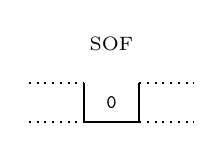
\begin{tikzpicture}
    \startcanbit
    \candots
    \draw (1.5 * \canbitwidth, 1) node {\cancommentstyle SOF} ;
    \canbitl{0}
    \candots
  \end{tikzpicture}
  \caption{Début de trame}
  \labelFigure{figureDebutTrame}
\end{figure}

Une trame commence par l'émission d'un bit dominant ($0$), le bit \texttt{SOF} (« \emph{Start of Frame} »). Le champ qui précède est un champ \texttt{IDLE} (bus au repos), qui a une durée quelconque qui n'est pas un multiple de la durée d'un bit. Aussi, les contrôleurs CAN en réception peuvent être complètement désynchronisés par rapport au contrôleur CAN en émission. Les contrôleurs CAN en réception réalisent donc une synchronisation forte (« \emph{Hard Synchronization} ») ; ce mécanisme sera étudié dans le \refChapterTitlePage{chapitreCalculBit}. Durant l'explication du format d'une trame, nous supposons qu'émetteur et récepteurs sont parfaitement synchronisés.










\subsection{Champs arbitrage, de contrôle (« \emph{Arbitration, Control Fields}~»)}

Ces deux champs sont décrits simultanément pour être plus facilement compréhensibles. Leur composition est illustrée par la \refFigure{}{figureChampArbitrage}. La composition du champ arbitrage peut paraître étrange et bizarremment compliquée. Mais cela s'explique pour des raisons historiques qui vont être exposées.

\begin{figure}[ht]
  \centering
  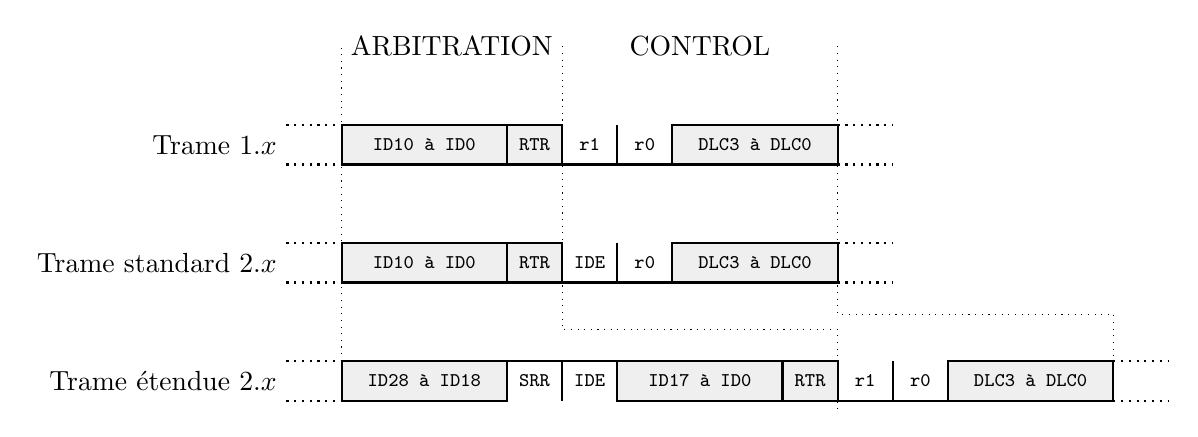
\begin{tikzpicture}
    \draw (\canbitwidth, 0)[dotted] -- ++ (0, 4.5) ;
    \draw (3 * \canbitwidth, 4.5) node {ARBITRATION} ;
    \draw (7.5 * \canbitwidth, 4.5) node {CONTROL} ;
    \draw (5 * \canbitwidth, 4.5)[dotted]
       -- (5 * \canbitwidth, 0.75 + .5 * \canbitheight - 0.1)
       -- ++ (5 * \canbitwidth, 0)
       -- ++ (0, -0.75 - .5 * \canbitheight) ;
    \draw (10 * \canbitwidth, 4.5)[dotted]
       -- (10 * \canbitwidth, 0.75 + .5 * \canbitheight + 0.1)
       -- ++ (5 * \canbitwidth, 0)
       -- ++ (0, -0.75 - .5 * \canbitheight) ;
    \draw (0, 3 + \canbitheight * .5) node [left] {Trame $1.x$} ;
    \draw (0, 1.5 + \canbitheight * .5) node [left] {Trame standard $2.x$} ;
    \draw (0, \canbitheight * .5) node [left] {Trame étendue $2.x$} ;
    \begin{scope}[yshift=3cm]
      \startcanbit
      \candots
      \canbitfield{ID10 à ID0}
      \canbit{RTR}
      \canbitl{r1}
      \canbitl{r0}
      \canbitfield{DLC3 à DLC0}
      \candots
    \end{scope}
    \begin{scope}[yshift=1.5cm]
      \startcanbit
      \candots
      \canbitfield{ID10 à ID0}
      \canbit{RTR}
      \canbitl{IDE}
      \canbitl{r0}
      \canbitfield{DLC3 à DLC0}
      \candots
    \end{scope}
    \begin{scope}
      \startcanbit
      \candots
      \canbitfield{ID28 à ID18}
      \canbith{SRR}
      \canbith{IDE}
      \canbitfield{ID17 à ID0}
      \canbit{RTR}
      \canbitl{r1}
      \canbitl{r0}
      \canbitfield{DLC3 à DLC0}
      \candots
    \end{scope}
  \end{tikzpicture}
  \caption{Champ arbitrage et champ de contrôle}
  \labelFigure{figureChampArbitrage}
\end{figure}

La première version du bus CAN ne définissait qu'un seul type de trame (« \emph{Trame 1.x} » sur la \refFigure{}{figureChampArbitrage}), et la composition des champs « \emph{ARBITRATION} » et « \emph{CONTROL} »  était simple et logique : $12$ bits pour le premier (les $11$ bits de l'identificateur et le bit \texttt{RTR}), $6$ bits pour le second (les deux bits \texttt{r1} et \texttt{r0} à $0$ suivis des quatre bits du champ \texttt{DLC}.

Le bit \texttt{RTR} (« \emph{Remote Transmission Request} ») est le bit qui permet de distinguer une trame de requête (\texttt{RTR} est à $1$), d'une trame de données (\texttt{RTR} à $0$).

Les bits \texttt{r1} et \texttt{r0} sont toujours à $0$ et étaient réservés à des extensions futures.

Les quatre bits \texttt{DLC3} à \texttt{DLC0} codent le nombre d'octets de la trame suivant le \refTableau{codageDLC}. À noter qu'une trame CAN contient au plus huit octets de données, les codes correspondants aux valeurs $9$ à $15$ sont invalides.

\begin{table}[!t]
  \small
  \centering
  \begin{tabular}{ccccl}
    \textbf{DLC3}& \textbf{DLC2} & \textbf{DLC1} & \textbf{DLC0}  & \textbf{Nombre d'octets de la trame} \\
     0 & 0 & 0 & 0 & 0 \\
     0 & 0 & 0 & 1 & 1 \\
     0 & 0 & 1 & 0 & 2 \\
     0 & 0 & 1 & 1 & 3 \\
     0 & 1 & 0 & 0 & 4 \\
     0 & 1 & 0 & 1 & 5 \\
     0 & 1 & 1 & 0 & 6 \\
     0 & 1 & 1 & 1 & 7 \\
     1 & 0 & 0 & 0 & 8 \\
     1 & 0 & 0 & 1 & \emph{Invalide} \\
     1 & 0 & 1 & $x$ & \emph{Invalide} \\
     1 & 1 & $x$ & $x$ & \emph{Invalide} \\
   \end{tabular}
  \caption{Nombre d'octets de la trame, en fonction du champ \texttt{DLC}}
  \labelTableau{codageDLC}
  \ligne
\end{table}

Puis le retour d'expérience a montré que $11$ bits pour l'identificateur étaient insuffisants pour certaines applications. Aussi, pour la deuxième version du bus CAN, il a été décidé de porter le nombre de bits de l'identificateur à $29$ bits, tout en gardant la compatibilité avec les trames de la première version. La signification du bit \texttt{r1} de la première version a été changé : ce bit est maintenant nommé \texttt{IDE} et permet de distinguer deux types de trame, les trames \emph{standard} et les trames \emph{étendues}.

Les trames standard de la version 2 (« \emph{Trame standard $2.x$} » sur la \refFigure{}{figureChampArbitrage}) ont leur bit \texttt{IDE} à $0$, de façon qu'une trame standard $2.x$ soit identique à une trame $1.x$.

Les trames étendues de la version 2 (« \emph{Trame étendue $2.x$} » sur la \refFigure{}{figureChampArbitrage}) ont leur bit \texttt{IDE} à $1$ ; mais il n'a pas été possible de placer consécutivement les $29$ bits de l'identicateur étendu : les $11$ bits de poids fort \texttt{ID28} à \texttt{ID18} sont d'abord transmis, puis, après le bit \texttt{IDE}, les $17$ bits de poids faible \texttt{ID17} à \texttt{ID0}. Le bit \texttt{SRR} (« \emph{SUBSTITUTE RTR BIT} ») est toujours à $1$  et doit être considéré comme réservé pour extension future.






\subsection{Champ \emph{de données} (« Data Field »)}

Si le bit \texttt{RTR} (« \emph{Remote Transmission Request} ») est à $1$, la trame est une trame de requête, et ce champ est toujours vide, quelque soit la valeur contenue dans le champ \texttt{DLC}.

Si le bit \texttt{RTR} est à $0$, la trame est une trame de données, et ce champ contient les octets de données, en fonction de la valeur contenue dans le champ \texttt{DLC} (\refTableau{codageDLC}). Comme le montre la \refFigure{}{figureChampDATA}, les octets sont transmis dans l'ordre \texttt{$D_0$}, ..., \texttt{$D_N$}, chaque octet étant transmis en commençant par le poids fort.



\begin{figure}[ht]
  \centering
  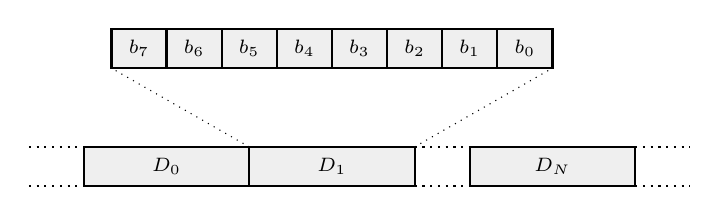
\begin{tikzpicture}
    \draw (4 * \canbitwidth, \canbitheight)[dotted] -- (1.5 * \canbitwidth, 1.5) ;
    \draw (7 * \canbitwidth, \canbitheight)[dotted] -- (9.5 * \canbitwidth, 1.5) ;
    \begin{scope}[yshift=1.5cm]
      \startcanbit
      \canspace{1.5}
      \canbit{$b_7$}
      \canbit{$b_6$}
      \canbit{$b_5$}
      \canbit{$b_4$}
      \canbit{$b_3$}
      \canbit{$b_2$}
      \canbit{$b_1$}
      \canbit{$b_0$}
    \end{scope}
    \startcanbit
    \candots
    \canbitfield{$D_0$}
    \canbitfield{$D_1$}
    \candots
    \canbitfield{$D_N$}
    \candots
  \end{tikzpicture}
  \caption{Composition du champ \emph{DATA}}
  \labelFigure{figureChampDATA}
\end{figure}





\subsection{Champ somme de contrôle (« \emph{Cyclic Redundancy Check Field} »)}

Après le champ \texttt{DATA}, toute l'information utile de la trame est transmise. Comme celle-ci peut être corrompue, une somme de contrôle est transmise. 

La somme de contrôle est calculée par l'émetteur à partir des valeurs de l'identificateur et des données, puis transmise.

Chaque récepteur la recalcule à partir des valeurs de l'identificateur et des données reçues, puis la compare à la somme de contrôle reçue :
\begin{itemize}
  \item si somme recalculée et somme reçue sont égales, la trame reçue est considérée valide et acceptée ;
  \item sinon, la réception est considérée invalide et rejetée.
\end{itemize}

Chaque récepteur signale l'acceptation de la réception en activant le bit \texttt{ACK SLOT}, décrit à la \refSubsectionPage{champAcquittement}. Un récepteur signale qu'il rejette la trame reçue en émettant une trame d'erreur (\refChapterPage{chapitreGestionErreurs}).

Comme l'illustre la \refFigure{}{figureChampCRC}, le champ \texttt{CRC} est composé du sous-champ \texttt{CRC SEQUENCE} de $15$ bits, qui contient la somme de contrôle proprement dite ; il est suivi d'un bit à $1$, le \texttt{CRC DELIMITER} qui permet aux récepteurs d'avoir le temps de décider si la trame reçue est valide ou doit être rejetée.

\begin{figure}[ht]
  \centering
  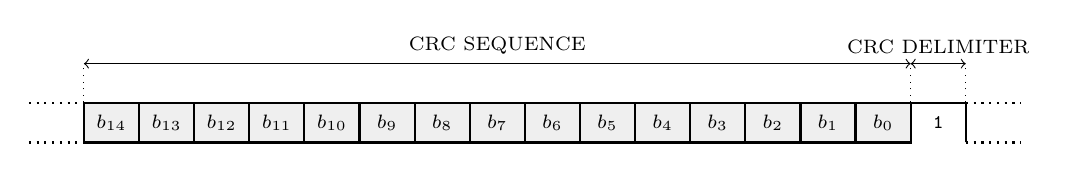
\begin{tikzpicture}
    \draw (\canbitwidth, 0)[dotted] -- ++ (0, 1) ;
    \draw (16 * \canbitwidth, 0)[dotted] -- ++ (0, 1) ;
    \draw (17 * \canbitwidth, 0)[dotted] -- ++ (0, 1) ;
    \draw (\canbitwidth, 1)[<->] -- ++ (15 * \canbitwidth, 0) node[midway, above]{\cancommentstyle CRC SEQUENCE} ;
    \draw (16 * \canbitwidth, 1)[<->] -- ++ (\canbitwidth, 0) ;
    \draw (16.5 * \canbitwidth, 1) node [above]{\cancommentstyle CRC DELIMITER} ;
    \startcanbit
    \candots
    \canbit{$b_{14}$}
    \canbit{$b_{13}$}
    \canbit{$b_{12}$}
    \canbit{$b_{11}$}
    \canbit{$b_{10}$}
    \canbit{$b_{9}$}
    \canbit{$b_{8}$}
    \canbit{$b_{7}$}
    \canbit{$b_{6}$}
    \canbit{$b_{5}$}
    \canbit{$b_{4}$}
    \canbit{$b_{3}$}
    \canbit{$b_{2}$}
    \canbit{$b_{1}$}
    \canbit{$b_{0}$}
    \canbith{1}
    \candots
  \end{tikzpicture}
  \caption{Composition du champ \emph{CRC}}
  \labelFigure{figureChampCRC}
\end{figure}


La technique utilisée pour calculer la somme de contrôle est celle des \emph{codes cycliques} : elle présente le double intérêt d'être très efficace et d'être facilement réalisable à partir de registres à décalage et de portes \emph{ou-exclusif}. Il existe une infinité de codes cycliques, chacun étant caractérisé par un polynome : celui utilisé par les contrôleurs CAN est $X^{15}+X^{14}+X^{10}+X^8+X^7+X^4+X^3+1$. La probabilité qu'une trame erronée vérifie la somme de contrôle est très faible\footnote{Unruh, J., Mathony, H.J., Kaiser, K.H.: Error Detection Analysis of Automotive Communication Protocols, SAE International Congress 1990.}, et évaluée à $4,7 \times 10^{-11}$.




\subsectionLabel{Champ d'acquittement (« \emph{Acknowledge Field} »)}{champAcquittement}

Le champ d'acquittement (\refFigure{}{figureChampACK}) est composé de deux bits, le bit \texttt{ACK SLOT} et le bit \texttt{ACK DELIMITER} qui est toujours à $1$.

\begin{figure}[ht]
  \centering
  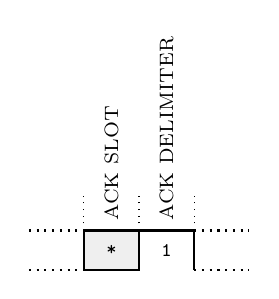
\begin{tikzpicture}
    \draw (\canbitwidth, 0)[dotted] -- ++ (0, 1) ;
    \draw (2 * \canbitwidth, 0)[dotted] -- ++ (0, 1) ;
    \draw (3 * \canbitwidth, 0)[dotted] -- ++ (0, 1) ;
    \draw (1.5 * \canbitwidth, \canbitheight) node [right, rotate=90]{\cancommentstyle ACK SLOT} ;
    \draw (2.5 * \canbitwidth, \canbitheight) node [right, rotate=90]{\cancommentstyle ACK DELIMITER} ;
    \startcanbit
    \candots
    \canbit{*}
    \canbith{1}
    \candots
  \end{tikzpicture}
  \caption{Composition du champ \emph{ACK}}
  \labelFigure{figureChampACK}
\end{figure}

Le bit \texttt{ACK SLOT} présente une particularité unique, c'est pour cela qu'il est représenté par une étoile dans la \refFigure{}{figureChampACK} :
\begin{itemize}
  \item l'émetteur émet toujours un bit récessif ($1$) ;
  \item chaque récepteur qui accepte la trame reçue émet un bit dominant ($0$).
\end{itemize}

Noter qu'un contrôleur CAN en réception émet des bits récessifs pendant la durée de la trame, sauf lors du bit \texttt{ACK SLOT} si il accepte la trame, et lorsqu'il a détecté une erreur.

Ainsi, lorsqu'un contrôleur transmet une trame, il envoie un bit récessif pour le bit \texttt{ACK SLOT}, et, si il est seul sur le bus, reçoit à cet emplacement un bit récessif, puisqu'aucun contrôleur sur le bus n'envoie de bit dominant. Cette situation peut être considérée comme une erreur par l'émetteur (voir \pasFini).

Si il y a un plusieurs contrôleurs CAN en réception, certains peuvent accepter la trame, d'autres la rejeter. Tous ceux qui acceptent envoient un bit dominant pour le bit \texttt{ACK SLOT}. L'émetteur reçoit donc un bit dominant, ce qui signifie qu'au moins un récepteur a accepté la trame. Mais il peut pas savoir combien ont accepté la trame. Ceux qui rejettent la trame envoient une trame d'erreur.




\subsection{Fin de la trame (« End of Frame »)}

Le champ \texttt{END OF FRAME} (\refFigure{}{figureChampEOF}) est constitué de $7$ bits récessifs. Si un contrôleur CAN en réception a détecté une erreur, il émet une trame d'erreur qui écrase ce champ.


\begin{figure}[ht]
  \centering
  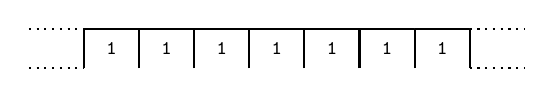
\begin{tikzpicture}
    \startcanbit
    \candots
    \canbith{1}
    \canbith{1}
    \canbith{1}
    \canbith{1}
    \canbith{1}
    \canbith{1}
    \canbith{1}
    \candots
  \end{tikzpicture}
  \caption{Composition du champ \emph{END OF FRAME}}
  \labelFigure{figureChampEOF}
\end{figure}


\subsection{Espace inter-trames (« \emph{Interframe Space} »)}

Le champ \texttt{INTERFRAME SPACE} commence par le champ \texttt{INTERMISSION} (trois bits récessifs, qui peuvent être écrasés par une trame d'erreur émise par un récepteur \pasFini), et est suivi par le champ \texttt{IDLE}.

\begin{figure}[ht]
  \centering
  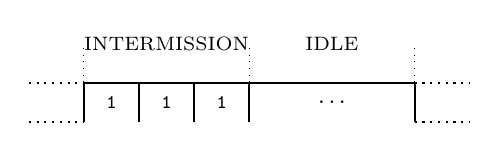
\begin{tikzpicture}
    \draw (\canbitwidth, 0)[dotted] -- ++ (0, 1) ;
    \draw (4 * \canbitwidth, 0)[dotted] -- ++ (0, 1) ;
    \draw (2.5 * \canbitwidth, 1) node {\cancommentstyle INTERMISSION} ;
    \draw (7 * \canbitwidth, 0) [dotted] -- ++ (0, 1) ;
    \draw (5.5 * \canbitwidth, 1) node {\cancommentstyle IDLE} ;
    \startcanbit
    \candots
    \canbith{1}
    \canbith{1}
    \canbith{1}
    
    \canidle
    \candots
  \end{tikzpicture}
  \caption{Composition de l'espace inter-trames « \emph{INTERFRAME SPACE} »}
  \labelFigure{figureChampInterframeSpace}
\end{figure}

Le sous-champ \texttt{IDLE} a une longueur quelconque :
\begin{itemize}
  \item nulle si une autre trame est émise (par le même contrôleur CAN ou par un autre) ; le champ \texttt{SOF} de la nouvelle trame suit directement le sous-champ \texttt{INTERMISSION} de la trame qui se termine ;
  \item si aucun contrôleur CAN ne désire émettre une trame, le bus CAN passe à l'état récessif, et le champ \texttt{IDLE} a une longueur quelconque, et ne sera interrompu que par le champ \texttt{SOF} d'une trame ; noter que durant l'état de repos, aucune synchronisation d'horloge n'a lieu entre les contrôleurs CAN du réseau, aussi la durée du champ \texttt{IDLE} n'au aucune raison d'être un multiple de la durée d'un bit.
\end{itemize}




\sectionLabel{Décision d'émettre : condition \emph{bus libre}}{decisionEmettre}

Quand un contrôleur CAN peut-il commencer à émettre une trame de données ?

Une trame en cours de transmission ne peut pas être préemptée : sa transmission doit se terminer avant qu'une autre ne soit transmise. Un contrôleur CAN voulant émettre doit donc surveiller le bus, et attendre qu'il soit libre.

{\bf Un contrôleur CAN considère que le bus est libre si le bus est dans l’état récessif pendant 11 bits consécutifs.}

En examinant le format d'une trame CAN (\refFigurePage{}{figureFormatTrameDonnees}), on constate en effet que la fin d'une trame est constituée des champs \texttt{ACK DELIMITER}, \texttt{END OF FRAME} et \texttt{INTERMISSION} qui totalisent $11$ bits. Aussi un contrôleur CAN désirant émettre place son bit \texttt{SOF} dès la fin du champ \texttt{INTERMISSION}, le champ \texttt{IDLE} étant vide.

%Pourquoi 11 ?
%le bit stuffing (voir plus loin) garantit que durant l’émission d’un message il n’y a pas de séquence de plus de 5 bits consécutifs égaux, un contrôleur CAN peut s’apercevoir que le bus est occupé ;
%les exigences particulières de la fin des trames (champs ACK, EOF, INTERFRAME SPACE) imposent cette règle.
%
%Un contrôleur CAN sollicité par son processeur peut donc commencer à émettre dès qu’il détecte la condition de bus libre.

Mais l'énoncé ci-dessus de la condition bus libre pose a priori deux problèmes.

D'abord, que se passe-t'il si $11$ bits récessifs sont rencontrés au cours de la transmission de la trame ? Par exemple, si un identificateur standard est constitué de $11$ bits à $1$, ou les données comportent $11$ bits consécutifs ou plus à $1$ ? En fait, cette situation ne peut jamais arriver, quelque soient la valeur de l'identificateur ou des données : ces champs sont soumis au mécanisme du « \emph{bit stuffing} » qui garantit qu'il n'y ait jamais de séquence de plus de $5$ bits consécutifs de même polarité. Ce mécanisme est décrit à la \refSectionPage{descriptionBitStuffing}.

Ensuite, supposons que plusieurs contrôleurs CAN sont sollicités pour émettre une trame alors qu'une autre est en cours de transmission. Ces contrôleurs attendent tous la condition bus libre, et en même temps s'aperçoivent que le bus devient libre. Ils commencent donc à émettre leur bit \texttt{SOF} et leur identificateur simultanément : il en résulte une collision sur le bus. Le protocole CAN a évidemment prévu cette situation en instaurant une priorité entre les trames : la \refSectionPage{resolutionCollision} montre comment la trame la plus prioritaire sort indemne de la collision et est transmise comme si elle avait été la seule à être émise. 








\section{Synchronisation des contrôleurs en réception}

Il y a un autre problème, que le mécanisme du \emph{bit stuffing} présenté à la section suivante va aider à résoudre : celui de la synchronisation des contrôleurs en réception.

En effet, le bus CAN véhicule les données, mais pas d'horloge ; chaque contrôleur CAN possède donc sa propre horloge locale. Or deux horloges différentes ont des fréquences (légèrement) différentes. Par exemple, une horloge à Quartz a une précision d'environ $10^{-4}$, donc la différence relative entre deux horloges à Quartz de même fréquence peut atteindre $2\times10^{-4}$.

Les règles définies par le protocole CAN sont :
\begin{itemize}
\item {\bf lors de la réception d'un bit \texttt{SOF}, les contrôleurs CAN en réception effectuent une synchronisation forte (« \emph{Hard Synchronization} ») en utilisant la transition récessif vers dominant du signal \texttt{RxD} ;} 
\item {\bf durant la transmission d'une trame, les contrôleurs CAN en réception utilisent les transitions récessif vers dominant du signal \texttt{RxD} pour se resynchroniser.} 
\end{itemize}

\begin{figure}[ht]
  \centering
  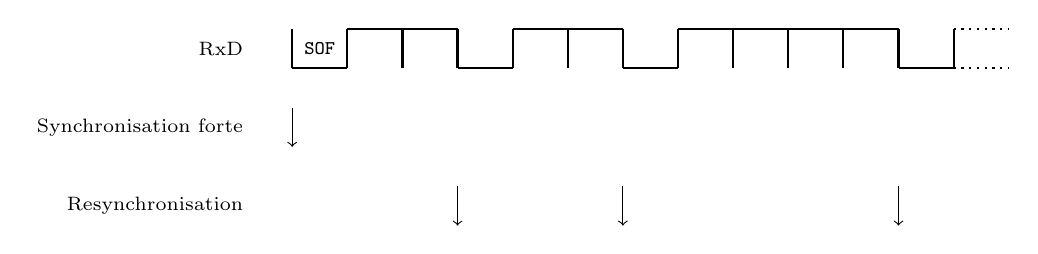
\begin{tikzpicture}
    \draw (-.5, .5 * \canbitheight) node[left] {\cancommentstyle RxD} ;
    \draw (-.5, -1.75) node[left] {\cancommentstyle Resynchronisation} ;
    \draw (-.5, -.75) node[left] {\cancommentstyle Synchronisation forte} ;
    \draw (0 * \canbitwidth, -.5) [->] -- ++ (0, -.5) ;
    \draw (3 * \canbitwidth, -1.5) [->] -- ++ (0, -.5) ;
    \draw (6 * \canbitwidth, -1.5) [->] -- ++ (0, -.5) ;
    \draw (11 * \canbitwidth, -1.5) [->] -- ++ (0, -.5) ;
    \startcanbit
    \canbitl{SOF}
    \canbith{}
    \canbith{}
    \canbitl{}
    \canbith{}
    \canbith{}
    \canbitl{}
    \canbith{}
    \canbith{}
    \canbith{}
    \canbith{}
    \canbitl{}
    \candots
  \end{tikzpicture}
  \caption{Synchronisation des contrôleurs en réception}
  \labelFigure{figureResynchronisation}
\end{figure}

Quand un émetteur émet un bit \texttt{SOF}, les récepteurs se synchronisent grâce au front descendant du signal \texttt{RxD}. Mais les différences relatives des fréquences d'horloge font que les récepteurs dérivent continuellement par rapport à l'émetteur : il faut donc que les récepteurs se resynchronisent régulièrement tout au long de la transmission d'une trame.

Lors de l'occurrence d'un top de resynchronisation, les contrôleurs en réception allongent ou raccourcissent leur durée de bit, de façon à rattraper ou attendre la phase du contrôleur en émission. Le mécanisme précis est décrit au \refChapterTitlePage{chapitreCalculBit}.











\sectionLabel{Le \emph{bit stuffing}}{descriptionBitStuffing}

{\bf Le « \emph{bit stuffing} » consiste pour le contrôleur en émission à intercaler après une séquence de cinq bits identiques un bit de polarité inverse. Ce mécanisme est actif depuis le champ \texttt{SOF} jusqu'au champ \texttt{CRC} inclus.}

Il est complètement transparent pour le programmeur, c'est-à-dire que le contrôleur effectue cette opération sans que l'on ait besoin de la programmer. À la réception, les bits insérés sont automatiquement éliminés.

La \refFigure{}{figureExemplesBitStuffing} montre quelques scénarios d'insertion de bits par ce mécanisme dans des trames standard. Les bits ainsi insérés sont notés \texttt{S}.

\begin{figure}[ht]
  \centering
  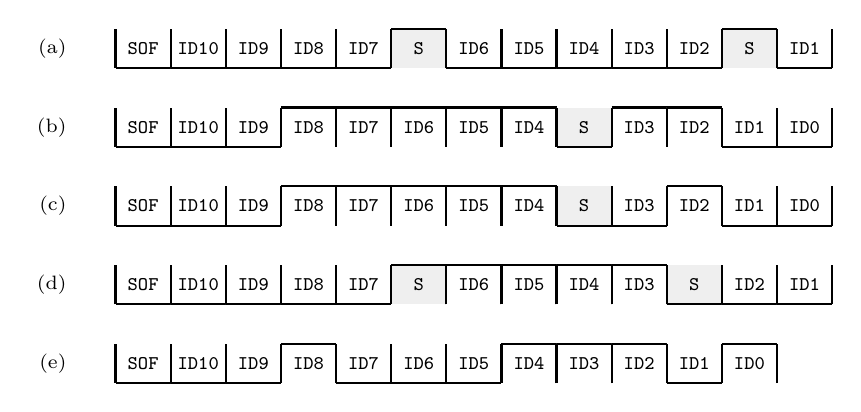
\begin{tikzpicture}
    \begin{scope}[yshift=4cm]
      \draw (-.5, .5 * \canbitheight) node[left] {\cancommentstyle (a)} ;
      \startcanbit
      \canbitl{SOF}
      \canbitl{ID10}
      \canbitl{ID9}
      \canbitl{ID8}
      \canbitl{ID7}
      \cangraybithigh{S}
      \canbitl{ID6}
      \canbitl{ID5}
      \canbitl{ID4}
      \canbitl{ID3}
      \canbitl{ID2}
      \cangraybithigh{S}
      \canbitl{ID1}
    \end{scope}
    \begin{scope}[yshift=3cm]
      \draw (-.5, .5 * \canbitheight) node[left] {\cancommentstyle (b)} ;
      \startcanbit
      \canbitl{SOF}
      \canbitl{ID10}
      \canbitl{ID9}
      \canbith{ID8}
      \canbith{ID7}
      \canbith{ID6}
      \canbith{ID5}
      \canbith{ID4}
      \cangraybitlow{S}
      \canbith{ID3}
      \canbith{ID2}
      \canbitl{ID1}
      \canbitl{ID0}
    \end{scope}
    \begin{scope}[yshift=2cm]
      \draw (-.5, .5 * \canbitheight) node[left] {\cancommentstyle (c)} ;
      \startcanbit
      \canbitl{SOF}
      \canbitl{ID10}
      \canbitl{ID9}
      \canbith{ID8}
      \canbith{ID7}
      \canbith{ID6}
      \canbith{ID5}
      \canbith{ID4}
      \cangraybitlow{S}
      \canbitl{ID3}
      \canbith{ID2}
      \canbitl{ID1}
      \canbitl{ID0}
    \end{scope}
    \begin{scope}[yshift=1cm]
      \draw (-.5, .5 * \canbitheight) node[left] {\cancommentstyle (d)} ;
      \startcanbit
      \canbitl{SOF}
      \canbitl{ID10}
      \canbitl{ID9}
      \canbitl{ID8}
      \canbitl{ID7}
      \cangraybithigh{S}
      \canbith{ID6}
      \canbith{ID5}
      \canbith{ID4}
      \canbith{ID3}
      \cangraybitlow{S}
      \canbitl{ID2}
      \canbitl{ID1}
    \end{scope}
    \begin{scope}
      \draw (-.5, .5 * \canbitheight) node[left] {\cancommentstyle (e)} ;
      \startcanbit
      \canbitl{SOF}
      \canbitl{ID10}
      \canbitl{ID9}
      \canbith{ID8}
      \canbitl{ID7}
      \canbitl{ID6}
      \canbitl{ID5}
      \canbith{ID4}
      \canbith{ID3}
      \canbith{ID2}
      \canbitl{ID1}
      \canbith{ID0}
    \end{scope}
  \end{tikzpicture}
  \caption{Exemples d'insertion de bit par le mécanisme de « \emph{bit stuffing} »}
  \labelFigure{figureExemplesBitStuffing}
\end{figure}

Dans la \refFigure{a}{figureExemplesBitStuffing} est considéré le cas d'un identificateur égal à $0$ : tous les bits \texttt{ID10} à \texttt{ID0} sont nuls, donc émis dominants. L'émission de la trame commence donc par cinq bits dominants : \texttt{SOF}, \texttt{ID10} à \texttt{ID7}. Le mécanisme de « \emph{bit stuffing} » insère donc un bit récessif après \texttt{ID7}. Ensuite, cinq nouveaux bits dominants sont transmis : \texttt{ID6} à \texttt{ID2} ; un nouveau bit récessif est donc inséré après \texttt{ID2}.

L'identificateur de la \refFigure{b}{figureExemplesBitStuffing} présente cinq bits consécutifs récessifs -- \texttt{ID8} à \texttt{ID4} -- le mécanisme de « \emph{bit stuffing} » insère donc un bit dominant après \texttt{ID4}. À noter que l'insertion d'un bit est décidé quand une séquence de cinq consécutifs de même polarité est rencontrée (ici \texttt{ID8} à \texttt{ID4}), sans tenir de la polarité du bit suivant (ici \texttt{ID3}). Autrement dit, il y a insertion d'un bit dominant après \texttt{ID4} même si \texttt{ID3} est dominant, ce qui est illustré par la \refFigure{c}{figureExemplesBitStuffing}.

La \refFigure{d}{figureExemplesBitStuffing} montre que le bit inséré par le mécanisme de « \emph{bit stuffing} » intervient dans le décompte des cinq bits consécutifs de même polarité. 


Enfin, la \refFigure{e}{figureExemplesBitStuffing} illustre le cas d'un identificateur pour lequel aucun bit n'a besoin d'être ajouté.

Pour terminer, la \refFigure{}{figureExempleInsertionMaxBitStuffing} montre un scénario d'insertion maximum de bits \texttt{S}. L'identificateur a une valeur telle que trois bits doivent être insérés durant sa transmission.

\begin{figure}[ht]
  \centering
  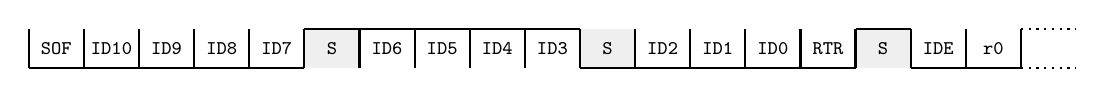
\begin{tikzpicture}
      \startcanbit
      \canbitl{SOF}
      \canbitl{ID10}
      \canbitl{ID9}
      \canbitl{ID8}
      \canbitl{ID7}
      \cangraybithigh{S}
      \canbith{ID6}
      \canbith{ID5}
      \canbith{ID4}
      \canbith{ID3}
      \cangraybitlow{S}
      \canbitl{ID2}
      \canbitl{ID1}
      \canbitl{ID0}
      \canbitl{RTR}
      \cangraybithigh{S}
      \canbitl{IDE}
      \canbitl{r0}
    \candots
  \end{tikzpicture}
  \caption{Scénario d'insertion maximum de bits par le « \emph{bit stuffing} »}
  \labelFigure{figureExempleInsertionMaxBitStuffing}
\end{figure}



\section{Longueur des trames CAN}

Une conséquence du mécanisme de « \emph{bit stuffing} » est que la longueur d'une trame dépend non seulement de son type (standard / étendue, données / requête) et du nombre d'octets de données ($0$ à $8$), mais aussi de la valeur de l'identificateur et des données.

Le \refTableau{codageLongueurTrames} donne la borne inférieure et supérieure de la longueur de chaque type de trame, exprimée en nombre de bits.
 
\begin{table}[!t]
  \small
  \centering
  \begin{tabular}{cccc}
    \textbf{Type de trame}& \textbf{Champ DLC} & \textbf{Longueur minimum} & \textbf{Longueur maximum} \\
    Requête Standard & 0 à 8 & 47 & 55 \\
    Donnée Standard & 0 & 47 & 55 \\
             & 1 & 55 & 65 \\
             & 2 & 63 & 75 \\
             & 3 & 71 & 85 \\
             & 4 & 79 & 95 \\
             & 5 & 87 & 105 \\
             & 6 & 95 & 115 \\
             & 7 & 103 & 125 \\
             & 8 & 111 & 135 \\
    Requête étendue  & 0 à 8 & 67 & 80 \\
    Donnée étendue  & 0 & 67 & 80 \\
             & 1 & 75 & 90 \\
             & 2 & 83 & 100 \\
             & 3 & 91 & 110 \\
             & 4 & 99 & 120 \\
             & 5 & 107 & 130 \\
             & 6 & 115 & 140 \\
             & 7 & 123 & 150 \\
             & 8 & 131 & 160 \\
   \end{tabular}
  \caption{Longueur d'une trame CAN, en fonction de son type et du champ \texttt{DLC}}
  \labelTableau{codageLongueurTrames}
  \ligne
\end{table}

Une trame de requête a la même taille qu'une trame de données sans données.

Pour une trame de données, les formules générales sont ($n$ étant le nombre d'octets de données, $s$ le nombre de bits ajoutés par le « \emph{bit stuffing} ») :
\begin{itemize}
  \item pour une trame standard de données : $47 + 8 \times n + s$, avec $0 \leqslant s \leqslant 8 + 2 \times n$ ;
  \item pour une trame étendue de données : $67 + 8 \times n + s$, avec $0 \leqslant s \leqslant 13 + 2 \times n$.
\end{itemize}

On peut facilement retrouver ces formules en se basant sur la description du format d'une trame de la \refFigurePage{}{figureFormatTrameDonnees}. Le \refTableau{calculLongueurTrames} donne la longueur minimum d'une trame de données contenant $n$ octets de données, en additionnant les longueurs minimum de chaque champ.





\begin{table}[!t]
  \small
  \centering
  \begin{tabular}{rrr}
    \textbf{Champ}& \textbf{Trame Standard} & \textbf{Trame étendue} \\
    SOF & $1$ & $1$ \\
    ARBITRATION & $12$ & $32$ \\
    CONTROL & $6$ & $6$ \\
    DATA & $8\times n$ & $8\times n$ \\
    CRC & $16$ & $16$ \\
    ACK & $2$ & $2$ \\
    EOF & $7$ & $7$ \\
    INTERMISSION & $3$ & $3$ \\
    {\bf Total :} & $47 + 8\times n$ & $67 + 8\times n$ \\
   \end{tabular}
  \caption{Calcul de la longueur minimum d'une trame de données}
  \labelTableau{calculLongueurTrames}
  \ligne
\end{table}

Pour le calcul de la valeur maximum de $s$, on remarque que les champs sujets au « \emph{bit stuffing} » s'étendent depuis le champ \texttt{SOF} jusqu'au champ \texttt{CRC} inclus (les champs \texttt{ACK}, \texttt{EOF} et \texttt{INTERMISSION} ne sont pas concernés), ce qui représente $35 + 8 \times n$ bits pour une trame standard de données, et $55 + 8 \times n$ bits pour une trame étendue de données. Quelle est la fréquence maximum d'insertion des bits \texttt{S} ? Le chronogramme de la \refFigure{d}{figureExemplesBitStuffing} indique qu'un bit \texttt{S} peut être inséré tous les quatre bits d'information. On obtient donc ainsi les bornes maximum de $s$ : $\frac{35 + 8 \times n}{4} = 8 + 2 \times n$ bits pour une trame standard de données, et $\frac{55 + 8 \times n}{4} = 13 + 2 \times n$ bits pour une trame étendue de données.

Mais ce calcul est pessimiste : il suppose que tous les bits des champs soumis au « \emph{bit stuffing} » puissent librement être dominants ou récessifs. Or, ce n'est pas le cas : les bits \texttt{RTR}, \texttt{SRR}, \texttt{r0}, \texttt{r1}, \texttt{CRC DELIMITER} ont des valeurs fixées ; toutes les combinaisons du champ \texttt{DLC} ne sont pas acceptées ; enfin, le champ \texttt{CRC SEQUENCE} a une valeur qui dépend uniquement de la valeur des champs qui le précèdent. Autrement dit, il se peut qu'il y ait aucune trame sans insertion de bit \texttt{S}, ou que le nombre maximum d'insertions ne soit jamais atteint. Les bornes énoncées dans le \refTableau{codageLongueurTrames} ne sont peut-être jamais atteintes.










\sectionLabel{Résolution des collisions}{resolutionCollision}

Les explications données jusqu'à présent dans ce chapitre supposent qu'il y a qu'un seul contrôleur CAN en émission à la fois. Dans cette section, le cas de plusieurs émissions simultanées va être étudié.

D'abord, dans quelle circonstance cette situation survient elle ? Rappelons le début de la \refSectionPage{decisionEmettre} :

\begin{tabular}{|l}
\begin{minipage}[flushright]{0.95\textwidth}
Une trame en cours de transmission ne peut pas être préemptée : sa transmission doit se terminer avant qu'une autre soit transmise. Un contrôleur CAN voulant émettre doit donc surveiller le bus, et attendre qu'il soit libre.

{\bf Un contrôleur CAN considère que le bus est libre si le bus est dans l’état récessif pendant 11 bits consécutifs.}
\end{minipage}
\end{tabular}


Considérons la situation suivante :
\begin{itemize}
  \item une trame est en cours de transmission ;
  \item durant cette transmission, trois contrôleurs désirent émettre chacun une trame ;
  \item ils attendent donc tous les trois la condition \emph{bus libre} ;
  \item à la fin de la transmission en cours, les trois contrôleurs s'aperçoivent en même temps que le bus devient libre ;
  \item en conséquence, les trois contrôleurs commencent à émettre leur trame en même temps : il en résulte une collision.
\end{itemize}


L'originalité du bus CAN est que la collision n'est pas destructive, la trame la plus prioritaire sortant indemne de la collision. La priorité entre les trames est donnée par la valeur de leur identificateurs :

{\bf Plus l'identificateur a une valeur numérique faible, plus la trame est prioritaire.}

Ainsi, pour des trames standard, la valeur $0$ est plus prioritaire que $1$, lui-même plus prioritaire que $2$, \dots, lui-même plus prioritaire que $2^{11}-1$. Il en est de même pour les trames étendues, l'identificateur le moins prioritaire étant $2^{29}-1$. La priorité relative entre une trame standard et une trame étendue est un peu long à décrire, ceci sera fait à la \refSectionPage{cohabitationStandardEtendue}.

La collision décrite ci-dessus est illustrée par la \refFigure{}{figureExempleArbitrage}. Bien que cette figure et les explications n'envisagent le cas d'une collision entre trois émissions de trames standard, le même mécanisme de résolution s'applique pour une collision entre un nombre quelconque d'émissions standard ou étendues. 


\begin{figure}[ht]
  \centering
  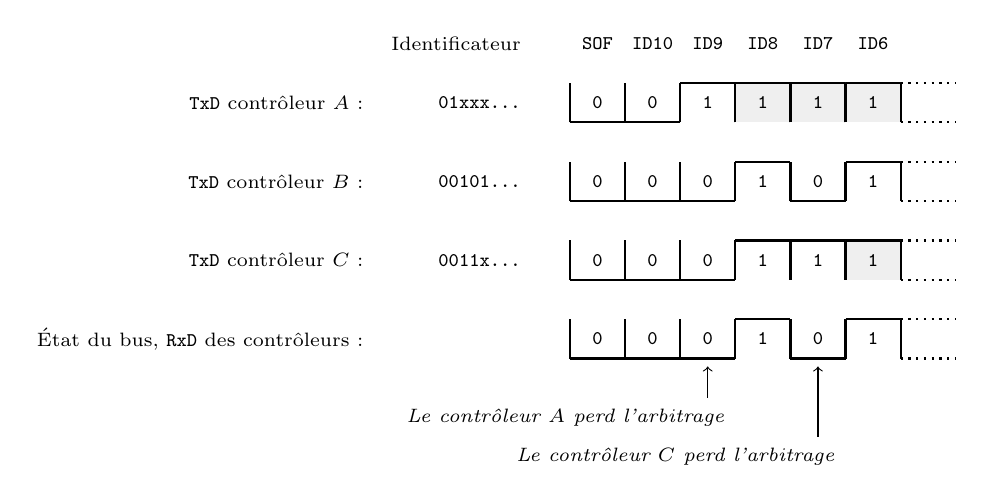
\begin{tikzpicture}
    \draw (-.5, 4) node[left] {\cancommentstyle Identificateur} ;
    \draw (.5 * \canbitwidth, 4) node {\cantextstyle SOF} ;
    \draw (1.5 * \canbitwidth, 4) node {\cantextstyle ID10} ;
    \draw (2.5 * \canbitwidth, 4) node {\cantextstyle ID9} ;
    \draw (3.5 * \canbitwidth, 4) node {\cantextstyle ID8} ;
    \draw (4.5 * \canbitwidth, 4) node {\cantextstyle ID7} ;
    \draw (5.5 * \canbitwidth, 4) node {\cantextstyle ID6} ;
    \begin{scope}[yshift=3cm]
      \draw (-2.5, .5 * \canbitheight) node[left] {\cancommentstyle \texttt{TxD} contrôleur $A$ :} ;
      \draw (-.5, .5 * \canbitheight) node[left] {\cantextstyle 01xxx\dots} ;
      \startcanbit
      \canbitl{0}
      \canbitl{0}
      \canbith{1}
      \cangraybithigh{1}
      \cangraybithigh{1}
      \cangraybithigh{1}
      \candots
    \end{scope}
    \begin{scope}[yshift=2cm]
      \draw (-2.5, .5 * \canbitheight) node[left] {\cancommentstyle \texttt{TxD} contrôleur $B$ :} ;
      \draw (-.5, .5 * \canbitheight) node[left] {\cantextstyle 00101\dots} ;
      \startcanbit
      \canbitl{0}
      \canbitl{0}
      \canbitl{0}
      \canbith{1}
      \canbitl{0}
      \canbith{1}
      \candots
    \end{scope}
    \begin{scope}[yshift=1cm]
      \draw (-2.5, .5 * \canbitheight) node[left] {\cancommentstyle \texttt{TxD} contrôleur $C$ :} ;
      \draw (-.5, .5 * \canbitheight) node[left] {\cantextstyle 0011x\dots} ;
      \startcanbit
      \canbitl{0}
      \canbitl{0}
      \canbitl{0}
      \canbith{1}
      \canbith{1}
      \cangraybithigh{1}
      \candots
    \end{scope}
    \begin{scope}
      \draw (-2.5, .5 * \canbitheight) node[left] {\cancommentstyle État du bus, \texttt{RxD} des contrôleurs :} ;
      \startcanbit
      \canbitl{0}
      \canbitl{0}
      \canbitl{0}
      \canbith{1}
      \canbitl{0}
      \canbith{1}
      \candots
    \end{scope}
  \draw (2.5 * \canbitwidth, -.1) [<-] -- ++ (0, -.4) ;
  \draw (3 * \canbitwidth, -.75) node[left] {\cancommentstyle \emph{Le contrôleur $A$ perd l'arbitrage}} ;
  \draw (4.5 * \canbitwidth, -.1) [<-] -- ++ (0, -.9) ;
  \draw (5 * \canbitwidth, -1.25) node[left] {\cancommentstyle \emph{Le contrôleur $C$ perd l'arbitrage}} ;
  \end{tikzpicture}
  \caption{Exemple d'arbitrage entre trois contrôleurs}
  \labelFigure{figureExempleArbitrage}
\end{figure}

Dans la \refFigure{}{figureExempleArbitrage}, Les trois contrôleurs émettent des trames dont seul le début des identificateurs est cité ; par exemple, pour le contrôleur $A$, l'identificateur est \texttt{01xxx\dots}, c'est-à-dire que \texttt{ID10} vaut $0$, \texttt{ID9} vaut $1$, et les bits suivants -- symbolisés par \texttt{x} ou des points de suspension -- n'ont pas d'importance pour la collision étudiée. Les chronogrammes montrent les lignes \texttt{TxD} des trois contrôleurs. La dernière ligne montre l'état du bus résultant de la collision des trois émissions, qui est un \emph{et} logique entre les trois signaux \texttt{TxD}; cet état est l'information qui remonte vers chaque contrôleur via sa ligne \texttt{RxD}.

{\bf Émission de \texttt{SOF}.} Chaque contrôleur émet un bit dominant ($0$), et reçoit un bit dominant. Tout est normal pour chaque contrôleur, qui ne sait même pas qu'il est compétition avec d'autres.

{\bf Émission de \texttt{ID10}.} Situation identique à la précédente.

{\bf Émission de \texttt{ID9}.} À ce moment, la situation évolue. Considérons d'abord les contrôleurs $B$ et $C$ : ils émettent un bit dominant, et reçoivent un bit dominant, rien n'a changé pour eux. Considérons d'abord le contrôleur $A$ : il émet un bit récessif ($1$), et reçoit un bit dominant : c'est l'indication pour lui qu'il vient de perdre la compétition, qu'il y a une ou plusieurs trames plus prioritaires qui sont en cours d'émission. Il acte sa défaite en renonçant à émettre sa trame immédiatement, et à partir de ce moment se met à envoyer des bits récessifs ($1$), qui ne perturberont pas l'émission en cours. Sur les chronogrammes de la \refFigure{}{figureExempleArbitrage}, ces bits apparaissent sur un fond gris.

{\bf Émission de \texttt{ID8}.} Chaque contrôleur émet un bit récessif, mais pour des raisons différentes : le contrôleur $A$ parce qu'il a perdu la compétition, et les contrôleurs $B$ et $C$ parce que cette valeur est celle du $8^e$ bit de leur identificateur. L'état du bus est récessif, chacun reçoit la valeur qu'il a émise : pas d'information nouvelle.


{\bf Émission de \texttt{ID7}.} Maintenant, $A$ émet toujours un bit récessif parce qu'il a perdu la compétition, $B$ un bit dominant, et $C$ un bit récessif. L'état résultant du bus est dominant. C'est maintenant $C$ qui envoie un récéssif et reçoit un dominant : à son tour, il perd la compétition, et, comme $A$ auparavant renonçe à émettre sa trame immédiatement, et se met à envoyer des bits récessifs.

{\bf Émission de \texttt{ID6}.}  À partir de cet instant, seul $B$ continue à transmettre sa trame : il a gagné la compétition : $B$ n'a jamais su qu'il était en compétition avec d'autres et les récepteurs ne savent pas qu'une compétition entre plusieurs émetteurs a eu lieu.

Donc, $B$ transmet sa trame, qui d'ailleurs peut être reçue par $A$ et par $C$ (et aussi par d'autres). À l'issue de cette transmission, le bus redeviendra libre, $A$ et $C$ entreront de nouveau en compétition. $C$ gagnera\footnote{À moins qu'un autre contrôleur entre dans la compétition avec une trame dont l'identificateur est plus prioritaire que celui de $C$.}, et émettra sa trame. Puis ce sera au tour de $A$ d'émettre sa trame.



\sectionLabel{Cohabitation des trames standards et étendues}{cohabitationStandardEtendue}

Un même réseau peut-il véhiculer trames standards et trames étendues ? Actuellement, la réponse est positive, même si cela n'a pas toujours été le cas, pour des raisons qui vont être expliquées.

{\bf Contrôleurs version 1.} Ces contrôleurs ne connaissent pas l'existence de trames étendues : il ne peuvent évidemment pas les émettre, et leur réception provoque une erreur (réception d'un bit \texttt{r1} récessif alors qu'un bit dominant est attendu, voir \refFigurePage{}{figureChampArbitrage}). Ces contrôleurs ont pratiquement tous disparu aujourd'hui. On peut citer le \texttt{PCA82C200} de Philips, remplacé par le \texttt{SJA1000} à partir de l'année 2000.

{\bf Contrôleurs version 1, tolérants.} Ces contrôleurs ne peuvent pas émettre de trame étendues, mais laissent passer les trames étendues : ils ne peuvent pas les recevoir, mais ne signalent pas d'erreur. Ces contrôleurs ont aussi pratiquement tous disparu aujourd'hui.

{\bf Contrôleurs version 2.} Ces contrôleurs peuvent émettre et recevoir trames standards et trames étendues. Tous les contrôleurs actuels sont de cette nature.

Un point plus délicat à comprendre est la priorité relative entre trame standard et trame étendue\footnote{Entre deux trames standard, ou entre deux trames étendues, c'est la valeur de l'identificateur qui détermine la priorité : plus sa valeur est faible, plus la trame est prioritaire, voir \refSectionPage{resolutionCollision}.}. Pour illustrer le raisonnement, la \refFigure{}{figureChampArbitrageStandardEtendue} montre les champs \texttt{ARBITRATION} et \texttt{CONTROL} des trames standard et étendues\footnote{Ces champs apparaissent aussi dans la \refFigurePage{}{figureChampArbitrage}.}.

\begin{figure}[ht]
  \centering
  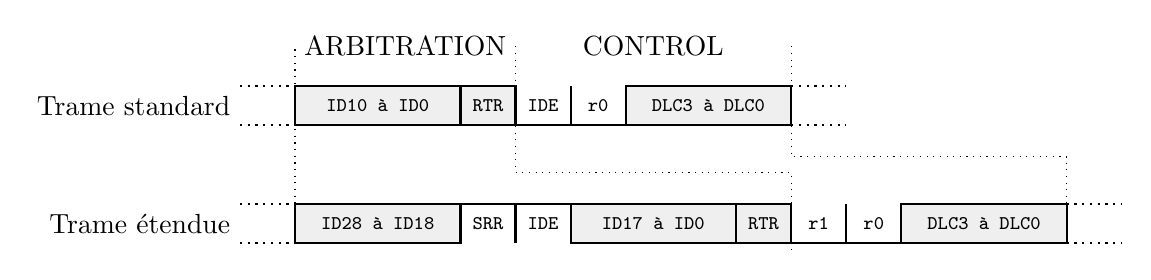
\begin{tikzpicture}
    \draw (\canbitwidth, 0)[dotted] -- ++ (0, 2.5) ;
    \draw (3 * \canbitwidth, 2.5) node {ARBITRATION} ;
    \draw (7.5 * \canbitwidth, 2.5) node {CONTROL} ;
    \draw (5 * \canbitwidth, 2.5)[dotted]
       -- (5 * \canbitwidth, 0.75 + .5 * \canbitheight - 0.1)
       -- ++ (5 * \canbitwidth, 0)
       -- ++ (0, -0.75 - .5 * \canbitheight) ;
    \draw (10 * \canbitwidth, 2.5)[dotted]
       -- (10 * \canbitwidth, 0.75 + .5 * \canbitheight + 0.1)
       -- ++ (5 * \canbitwidth, 0)
       -- ++ (0, -0.75 - .5 * \canbitheight) ;
    \draw (0, 1.5 + \canbitheight * .5) node [left] {Trame standard} ;
    \draw (0, \canbitheight * .5) node [left] {Trame étendue} ;
    \begin{scope}[yshift=1.5cm]
      \startcanbit
      \candots
      \canbitfield{ID10 à ID0}
      \canbit{RTR}
      \canbitl{IDE}
      \canbitl{r0}
      \canbitfield{DLC3 à DLC0}
      \candots
    \end{scope}
    \begin{scope}
      \startcanbit
      \candots
      \canbitfield{ID28 à ID18}
      \canbith{SRR}
      \canbith{IDE}
      \canbitfield{ID17 à ID0}
      \canbit{RTR}
      \canbitl{r1}
      \canbitl{r0}
      \canbitfield{DLC3 à DLC0}
      \candots
    \end{scope}
  \end{tikzpicture}
  \caption{Champ arbitrage et contrôle des trames standards et étendues}
  \labelFigure{figureChampArbitrageStandardEtendue}
\end{figure}

L'arbitrage commençant par les poids forts, il y a compétition entre l'identificateur de la trame standard et les onze bits de poids fort de l'identificateur de la trame étendue. La valeur la plus faible est la plus prioritaire. Si il y a égalité :
\begin{itemize}
  \item si la trame standard est une trame de données, son bit \texttt{RTR} est dominant ; comme le bit \texttt{SRR} est récessif, la trame standard est prioritaire ;
  \item si la trame standard est une trame de requête, son bit \texttt{RTR} est récessif, comme le bit \texttt{SRR} ; la décision ne peut pas être prise sur ce bit ;
  \item le bit \texttt{IDE} est dominant pour une trame standard, et récessif pour une trame étendue ; la trame standard est donc prioritaire.
\end{itemize}

La règle est donc la suivante : {\bf une trame étendue est plus prioritaire qu'une trame standard si le nombre formé par les onze bits de poids fort de l'identificateur de la trame étendue est strictement inférieur à la valeur de l'identificateur de la trame standard}.






\section{Trame de surcharge}

Pas à sa place ici, laissé pour mémoire. \cite{pasFini}


